\section{SimSite3D::Score\-Map\-Base Class Reference}
\label{classSimSite3D_1_1ScoreMapBase}\index{SimSite3D::ScoreMapBase@{SimSite3D::ScoreMapBase}}
{\tt \#include $<$Score\-Map\-Base.H$>$}

Inheritance diagram for SimSite3D::Score\-Map\-Base::\begin{figure}[H]
\begin{center}
\leavevmode
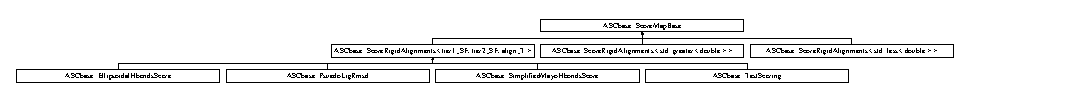
\includegraphics[height=0.88189cm]{classSimSite3D_1_1ScoreMapBase}
\end{center}
\end{figure}
\subsection*{Public Member Functions}
\begin{CompactItemize}
\item 
\bf{Score\-Map\-Base} (const \bf{Search\-Parameters} \&params)
\item 
virtual \bf{$\sim$Score\-Map\-Base} ()\label{classSimSite3D_1_1ScoreMapBase_53cc54d782902810408e5e4ebcbbffd5}

\begin{CompactList}\small\item\em basic destruction \item\end{CompactList}\item 
bool \bf{set\_\-external\_\-scoring\_\-method} (const std::string sf\_\-name, std::string method\_\-name)
\item 
template$<$class align\_\-mmap\_\-iter$>$ bool \bf{run\_\-external\_\-scoring\_\-method} (align\_\-mmap\_\-iter a\_\-beg, align\_\-mmap\_\-iter a\_\-end, const std::string \&prot\_\-fname, const std::string \&struct\_\-id, const std::string \&output\_\-dir)
\begin{CompactList}\small\item\em Run the external scoring function over all the saved alignments. \item\end{CompactList}\item 
void \bf{get\_\-ext\_\-SF\_\-names} (std::vector$<$ std::string $>$ $\ast$names)\label{classSimSite3D_1_1ScoreMapBase_b5ee9de7e756e9c6ee3058c475a95958}

\begin{CompactList}\small\item\em Get the name(s) of the external scoring function(s). \item\end{CompactList}\end{CompactItemize}
\subsection*{Protected Attributes}
\begin{CompactItemize}
\item 
std::string \textbf{A\_\-scratch\_\-dir}\label{classSimSite3D_1_1ScoreMapBase_784728589fd2db54ce16e5043db3c349}

\item 
bool \bf{A\_\-write\_\-ligands}\label{classSimSite3D_1_1ScoreMapBase_c11f067cce7e9e72f38b4cdc2abde485}

\begin{CompactList}\small\item\em True =$>$ write ligs and frags, else do not write. \item\end{CompactList}\item 
bool \bf{A\_\-prot\_\-lig\_\-score}\label{classSimSite3D_1_1ScoreMapBase_42d2d13e5fa5d7492495dd531246f8a5}

\begin{CompactList}\small\item\em True ==$>$ compute query prot -- dbase lig frag affi and orient scores. \item\end{CompactList}\item 
std::string \bf{ext\_\-SF\_\-id}\label{classSimSite3D_1_1ScoreMapBase_b6bfd4fcc3263c7ee1cc86c856cea184}

\begin{CompactList}\small\item\em Label given to the ext. prot-lig scoring fcn. \item\end{CompactList}\end{CompactItemize}
\subsection*{Private Attributes}
\begin{CompactItemize}
\item 
\bf{External\-Scoring\-Function} $\ast$ \bf{A\_\-external\_\-SF}\label{classSimSite3D_1_1ScoreMapBase_490667b180269340cbf0017b282eabb6}

\begin{CompactList}\small\item\em external prot-lig score fcn ptr \item\end{CompactList}\end{CompactItemize}


\subsection{Detailed Description}
Because of the gcc model, we must have all template definitions included in all the source files which use the functions, classes, etc that are prototyped and defined using the template keyword. 



\subsection{Constructor \& Destructor Documentation}
\index{SimSite3D::ScoreMapBase@{SimSite3D::Score\-Map\-Base}!ScoreMapBase@{ScoreMapBase}}
\index{ScoreMapBase@{ScoreMapBase}!SimSite3D::ScoreMapBase@{SimSite3D::Score\-Map\-Base}}
\subsubsection{\setlength{\rightskip}{0pt plus 5cm}SimSite3D::Score\-Map\-Base::Score\-Map\-Base (const \bf{Search\-Parameters} \& {\em params})\hspace{0.3cm}{\tt  [inline]}}\label{classSimSite3D_1_1ScoreMapBase_17c627b5ef8a777466b2f9ebc50bd228}


\begin{Desc}
\item[Parameters:]
\begin{description}
\item[{\em params}]Reference to the search's runtime parameters \end{description}
\end{Desc}


\subsection{Member Function Documentation}
\index{SimSite3D::ScoreMapBase@{SimSite3D::Score\-Map\-Base}!run_external_scoring_method@{run\_\-external\_\-scoring\_\-method}}
\index{run_external_scoring_method@{run\_\-external\_\-scoring\_\-method}!SimSite3D::ScoreMapBase@{SimSite3D::Score\-Map\-Base}}
\subsubsection{\setlength{\rightskip}{0pt plus 5cm}template$<$class align\_\-mmap\_\-iter$>$ bool SimSite3D::Score\-Map\-Base::run\_\-external\_\-scoring\_\-method (align\_\-mmap\_\-iter {\em a\_\-beg}, align\_\-mmap\_\-iter {\em a\_\-end}, const std::string \& {\em prot\_\-fname}, const std::string \& {\em struct\_\-id}, const std::string \& {\em output\_\-dir})\hspace{0.3cm}{\tt  [inline]}}\label{classSimSite3D_1_1ScoreMapBase_85708eaffffc9a4e36bbd7375b552586}


Run the external scoring function over all the saved alignments. 

For a given SimSite3D run, the model sitemap is held constant. Thus, we need only one protein\_\-file. For each saved alignment, score the protein and the saved ligand fragment.

\begin{Desc}
\item[Parameters:]
\begin{description}
\item[{\em protein\_\-file}]Protein PDB corresponding to the model sitemap \item[{\em output\_\-dir}]Directory holding the ligand fragments \end{description}
\end{Desc}
\begin{Desc}
\item[Returns:]True if the scoring function was initialized, else false \end{Desc}
\index{SimSite3D::ScoreMapBase@{SimSite3D::Score\-Map\-Base}!set_external_scoring_method@{set\_\-external\_\-scoring\_\-method}}
\index{set_external_scoring_method@{set\_\-external\_\-scoring\_\-method}!SimSite3D::ScoreMapBase@{SimSite3D::Score\-Map\-Base}}
\subsubsection{\setlength{\rightskip}{0pt plus 5cm}bool SimSite3D::Score\-Map\-Base::set\_\-external\_\-scoring\_\-method (const std::string {\em sf\_\-name}, std::string {\em method\_\-name})\hspace{0.3cm}{\tt  [inline]}}\label{classSimSite3D_1_1ScoreMapBase_d24ec72fca67bdacb134c71a0e78e9d6}


Setup the external scoring function. This function is in this class since it acts as a storage class for the alignments

\begin{Desc}
\item[Parameters:]
\begin{description}
\item[{\em sf\_\-name}]Path to the external scoring function file \item[{\em method\_\-name}]Name of the external scoring function (as stored in the external\_\-scoring\_\-functions.txt file) \end{description}
\end{Desc}
\begin{Desc}
\item[Returns:]True if method was found, else false \end{Desc}


The documentation for this class was generated from the following file:\begin{CompactItemize}
\item 
Score\-Map\-Base.H\end{CompactItemize}
